\documentclass{article}

\usepackage{graphicx}
\usepackage{rotating}
\usepackage{amsmath}
\usepackage{fancyhdr}
\usepackage{listings}
\usepackage{xcolor}
\usepackage{color}
\usepackage{textcomp}
\usepackage{float}
\usepackage{titlesec}
\usepackage[sorting=none]{biblatex}
\usepackage[margin=1in]{geometry}
\usepackage[font={small,it}]{caption}
\usepackage{placeins}
\usepackage{xepersian}

%\DeclareMathOperator*{\btie}{\bowtie}
\addbibresource{bibliography.bib}
\settextfont[Scale=1.2]{B-NAZANIN.TTF}
\setlatintextfont[Scale=1]{Times New Roman}
\renewcommand{\baselinestretch}{1.5}
\pagestyle{fancy}
\fancyhf{}
\rhead{پروژه‌ی دوم درس شبکه‌های کامپیوتری 2}
\lhead{\thepage}
\rfoot{علیرضا ابره فروش}
\lfoot{9816603}
\renewcommand{\headrulewidth}{1pt}
\renewcommand{\footrulewidth}{1pt}
%%%%%%%%%%
\lstset
{
    language=[latex]tex,
    basicstyle=\ttfamily,
    commentstyle=\color{black},
    columns=fullflexible,
    keepspaces=true,
    upquote=true,
    showstringspaces=false,
    morestring=[s]\\\%,
    stringstyle=\color{black},
}
%%%%%%%%%%
%beginMatlab
\definecolor{mygreen}{RGB}{28,172,0} % color values Red, Green, Blue
\definecolor{mylilas}{RGB}{170,55,241}
%endMatlab
\begin{document}
%beginMatlab
\lstset{language=Matlab,%
    %basicstyle=\color{red},
    breaklines=true,%
    morekeywords={matlab2tikz},
    keywordstyle=\color{blue},%
    morekeywords=[2]{1}, keywordstyle=[2]{\color{black}},
    identifierstyle=\color{black},%
    stringstyle=\color{mylilas},
    commentstyle=\color{mygreen},%
    showstringspaces=false,%without this there will be a symbol in the places where there is a space
    numbers=left,%
    numberstyle={\tiny \color{black}},% size of the numbers
    numbersep=9pt, % this defines how far the numbers are from the text
    emph=[1]{for,end,break},emphstyle=[1]\color{red}, %some words to emphasise
    %emph=[2]{word1,word2}, emphstyle=[2]{style},    
}
%endMatlab
\begin{titlepage}
\begin{center}

\includegraphics[width=0.4\textwidth]{figures/IUT Logo.png}\\
        
\LARGE
\textbf{دانشگاه صنعتی اصفهان}\\
\textbf{دانشکده مهندسی برق و کامپیوتر}\\
        
\vfill
        
\huge
\textbf{عنوان: تکلیف چهارم درس ریزپردازنده}\\
        
\vfill
        
\LARGE
\textbf{نام و نام خانوادگی: علیرضا ابره فروش}\\
\textbf{شماره دانشجویی: 9816603}\\
\textbf{نیم\,سال تحصیلی: پاییز 1400}\\
\textbf{مدرّس: دکتر عارف کریمی افشار}\\
\end{center}
\end{titlepage}


%\tableofcontents
\newpage




\section{}
\subsection{}
همانطور که در تصویر زیر می‌بینیم، بسته‌هایی که در وایرشارک کپچر شده‌اند از پروتکل‌های \lr{TCP}، \lr{OpenFlow} و \lr{DNS} استفاده کرده‌اند.
\begin{figure}[H]
    \centering
    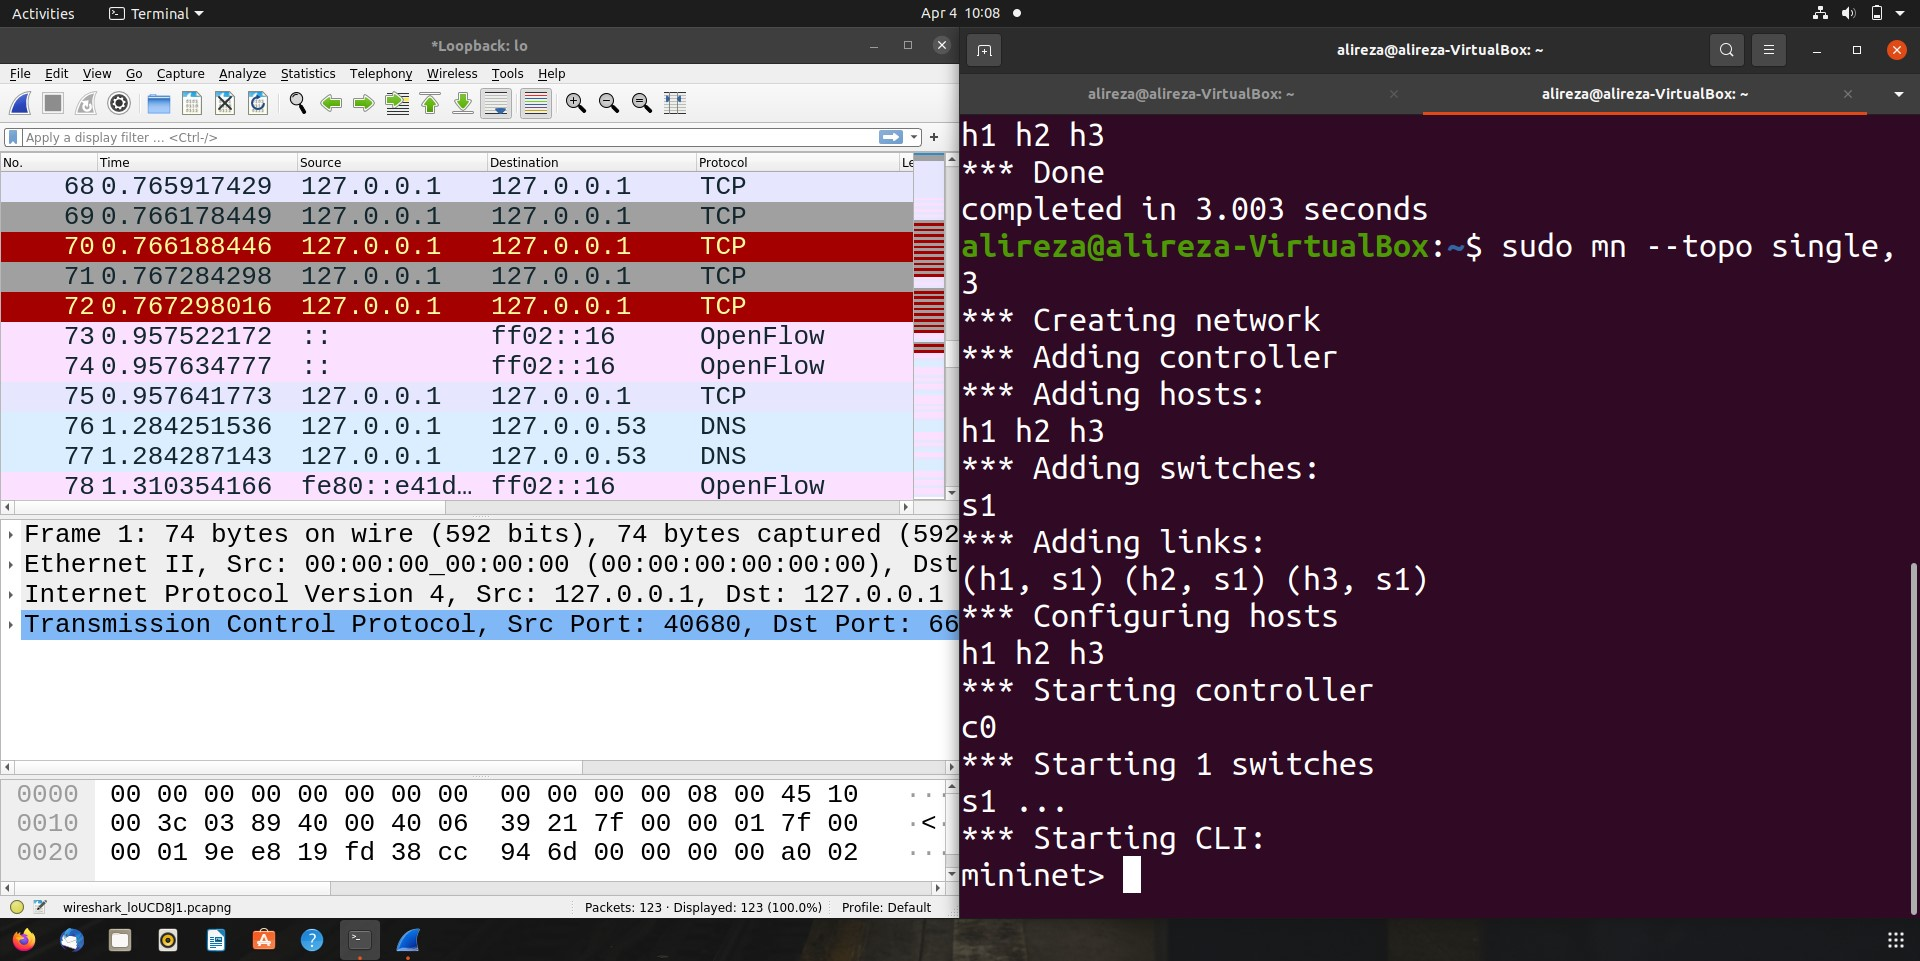
\includegraphics[width=1.0\textwidth]{figures/1a.jpg}
    \caption
	{
رصد پکت‌ها در وایرشارک
	}
    \label{fig:fig1}
\end{figure}

\subsection{}
\begin{figure}[H]
    \centering
    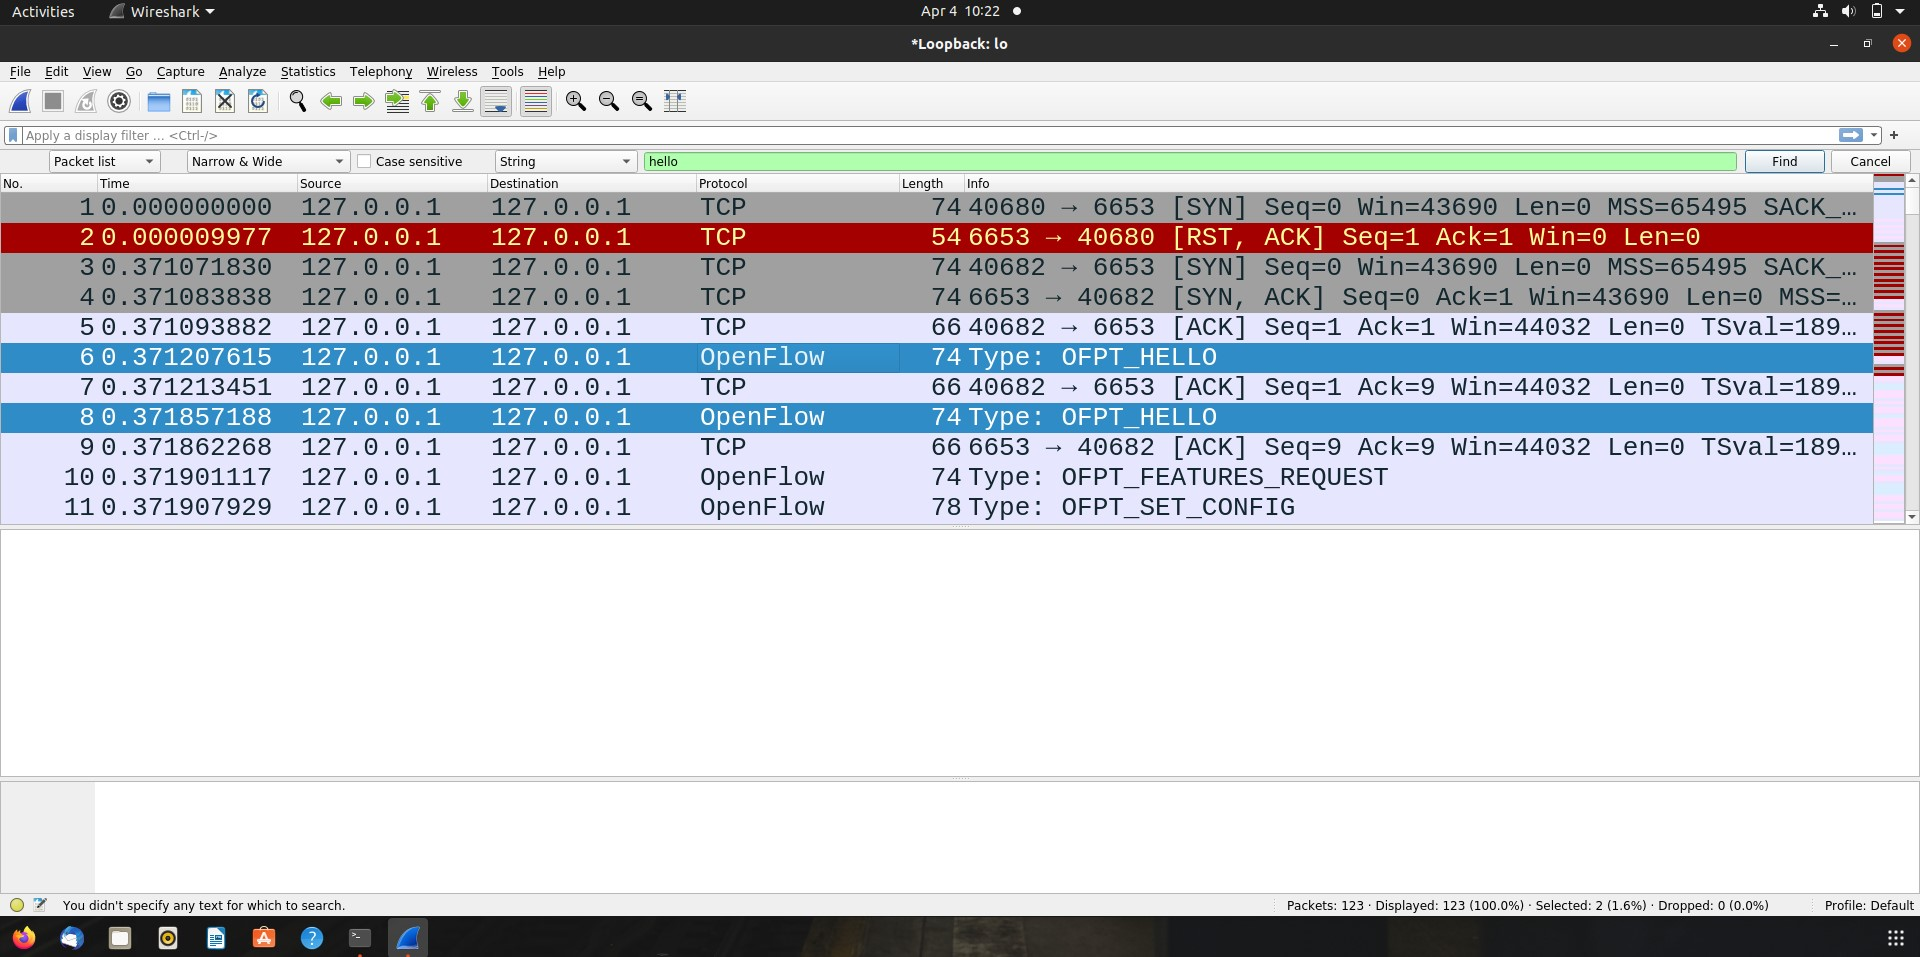
\includegraphics[width=1.0\textwidth]{figures/1b.jpg}
    \caption
	{
رد و بدل شدن پیغامِ \lr{Hello} بین سوئیچ و کنترلر در زمان‌های \lr{0.371207615} و \lr{0.371857188} ثانیه پس از اجرای دستور
	}
    \label{fig:fig1}
\end{figure}

\subsection{}
\begin{figure}[H]
    \centering
    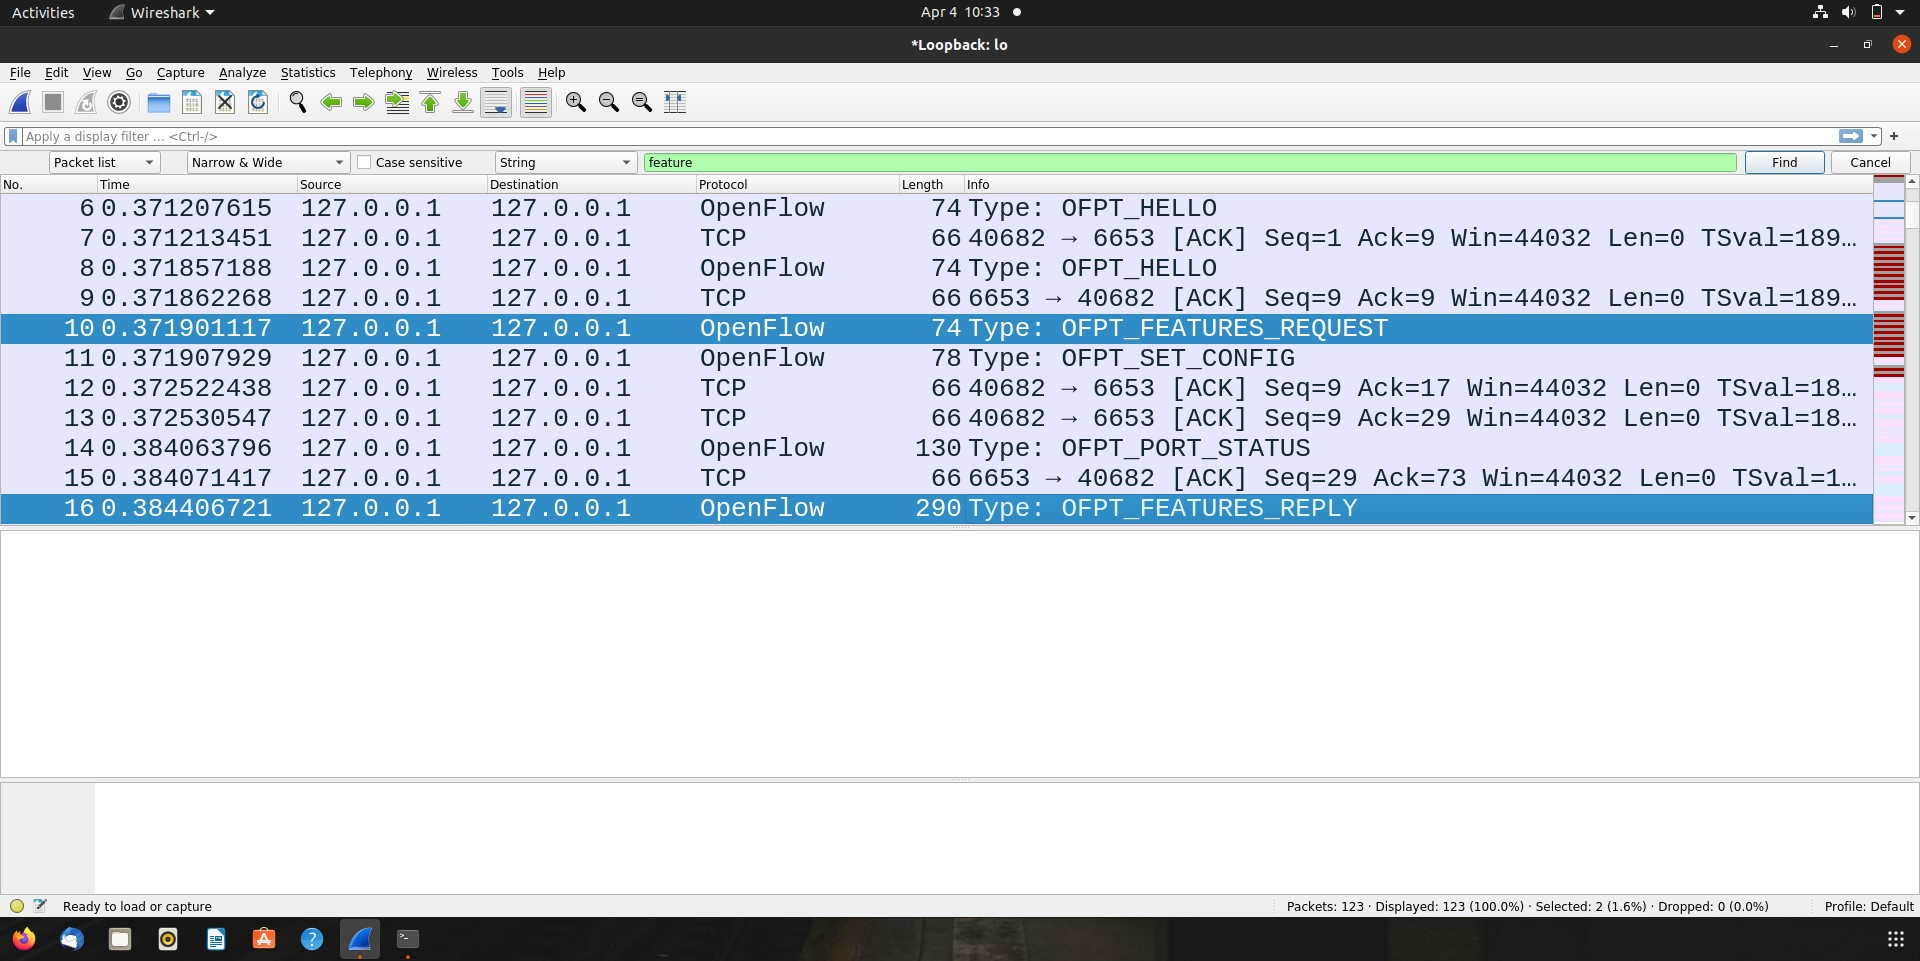
\includegraphics[width=1.0\textwidth]{figures/1c.jpg}
    \caption
	{
پیغام‌های \lr{Feature request} و \lr{Feature reply}
	}
    \label{fig:fig1}
\end{figure}

پیغام \lr{Feature request} توسط کنترلر به سوئیچ جهت گرفتن اطلاعات از قبیل \lr{datapath ID} ارسال می‌شود.
\begin{figure}[H]
    \centering
    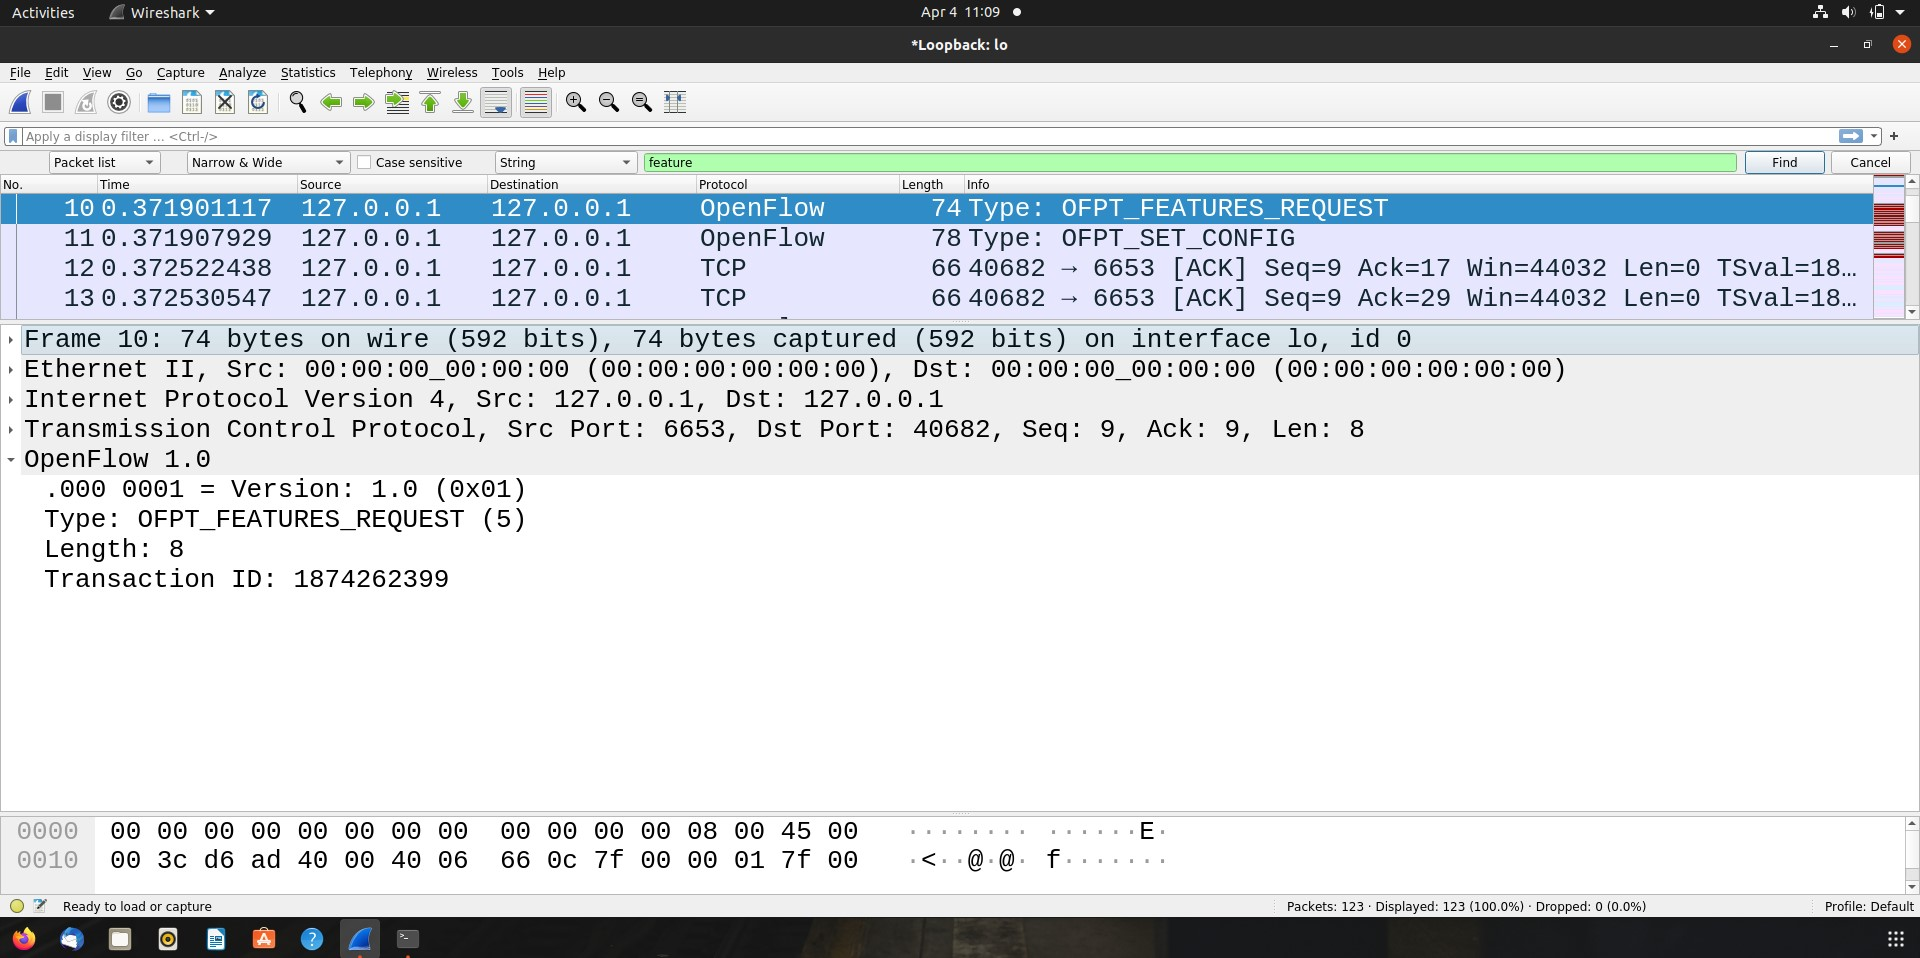
\includegraphics[width=1.0\textwidth]{figures/1e.jpg}
    \caption
	{
پیغام \lr{Feature request}
	}
    \label{fig:fig1}
\end{figure}
همانطور که در تصویر زیر می‌بینیم، پیغام \lr{Feature reply} حاویِ \lr{datapath ID}ِ یکتا و اطلاعات درباره‌ی پورت‌های سوئیچ شامل نام هر پورت می‌باشد. همچنین سایر اطلاعات مربوطه در این پیغام موجود است. پس از دریافت \lr{Feature request} توسط سوئیچ، اطلاعات خواسته شده را به کنترلر ارسال می‌کند.
\begin{figure}[H]
    \centering
    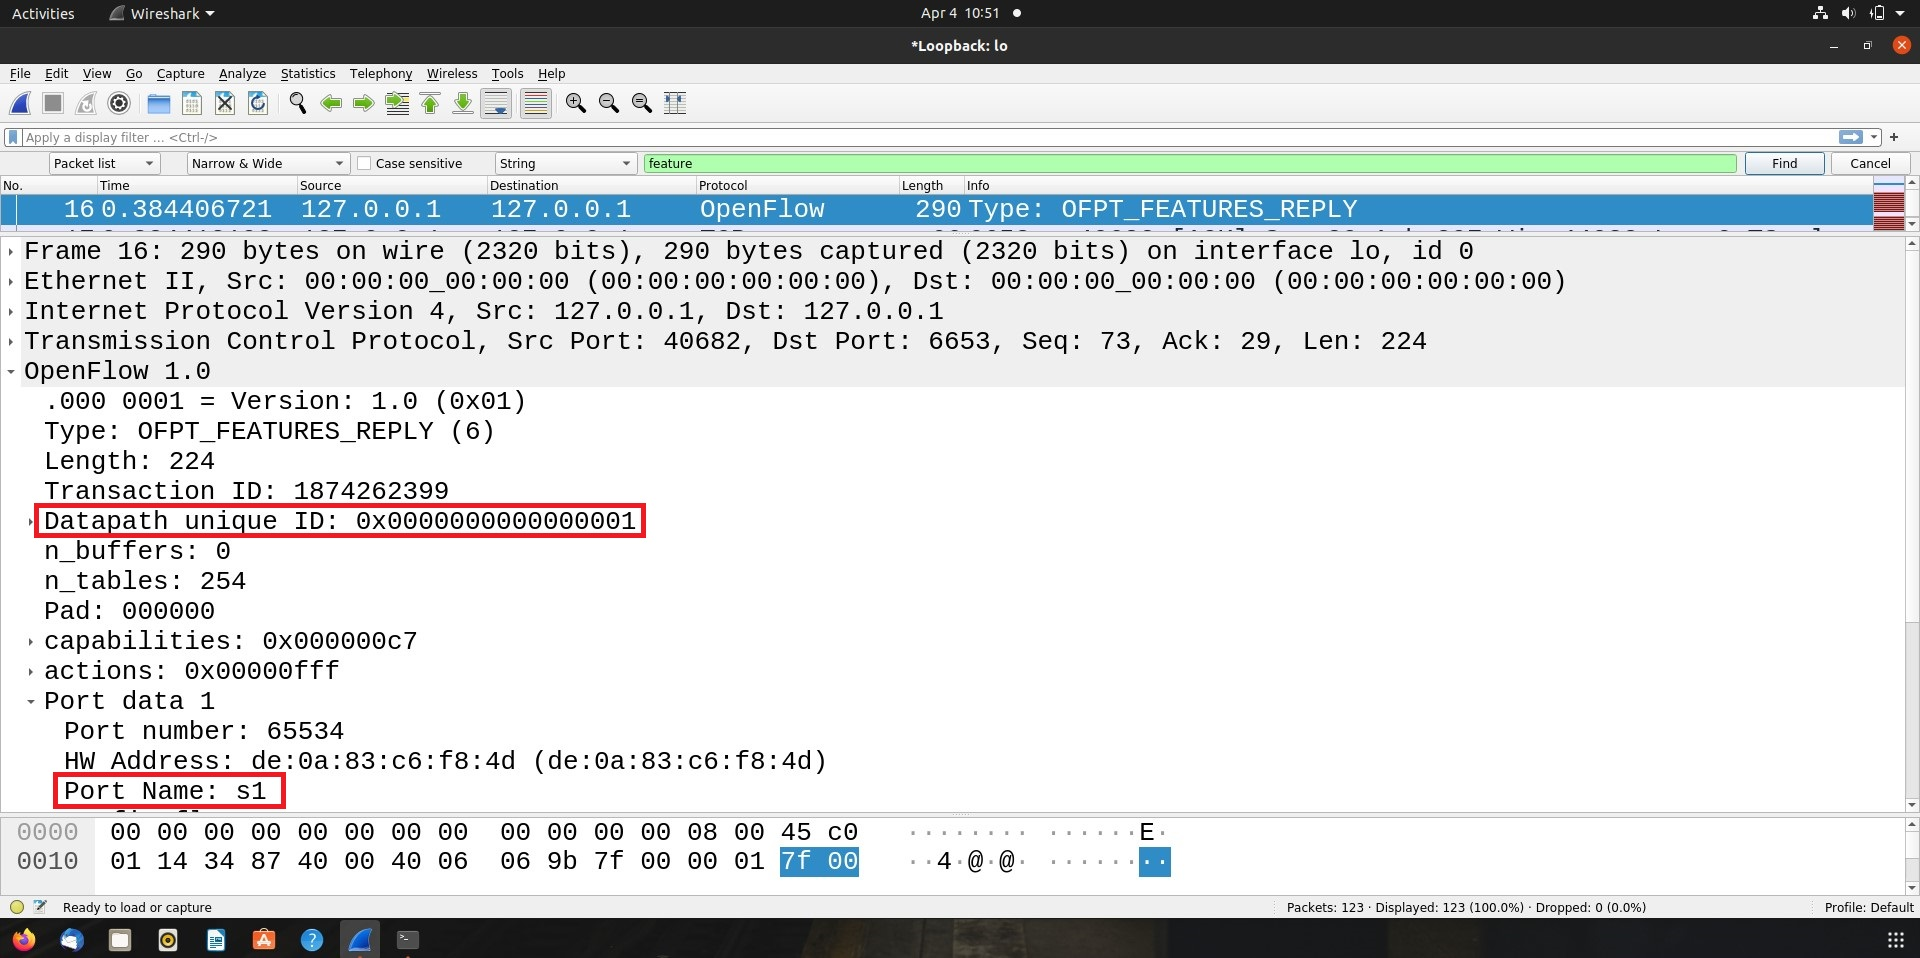
\includegraphics[width=1.0\textwidth]{figures/1d.jpg}
    \caption
	{
پیغام \lr{Feature reply}
	}
    \label{fig:fig1}
\end{figure}

\subsection{}
\begin{figure}[H]
    \centering
    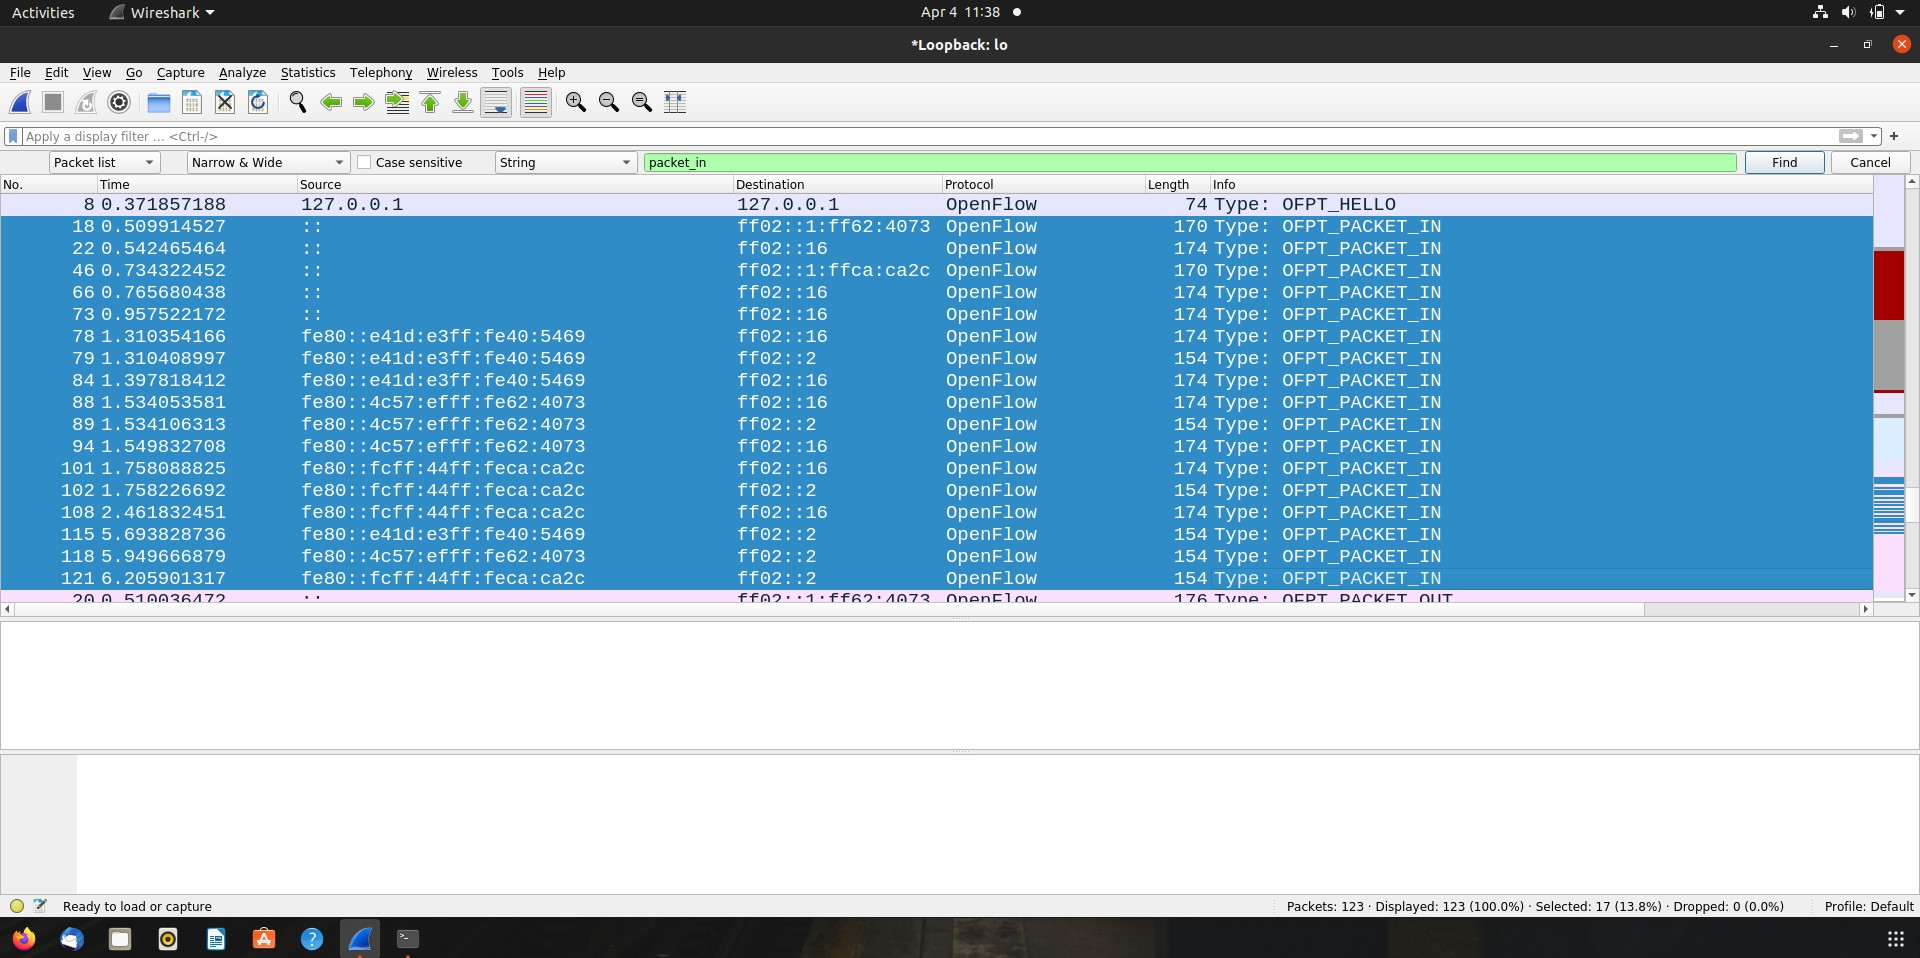
\includegraphics[width=1.0\textwidth]{figures/1f.jpg}
    \caption
	{
پیغام‌های \lr{Packet\_in}
	}
    \label{fig:fig1}
\end{figure}


\subsection{}
به ازای همه پکت‌هایی که یا \lr{matching flow entry} ندارند یا یک پکت با \lr{entry}ی با \lr{control action}ِ \lr{send to} \lr{match} شود، یک پیغامِ \lr{packet\_in} برای کنترلر ارسال می‌شود.

\subsection{}
\begin{figure}[H]
    \centering
    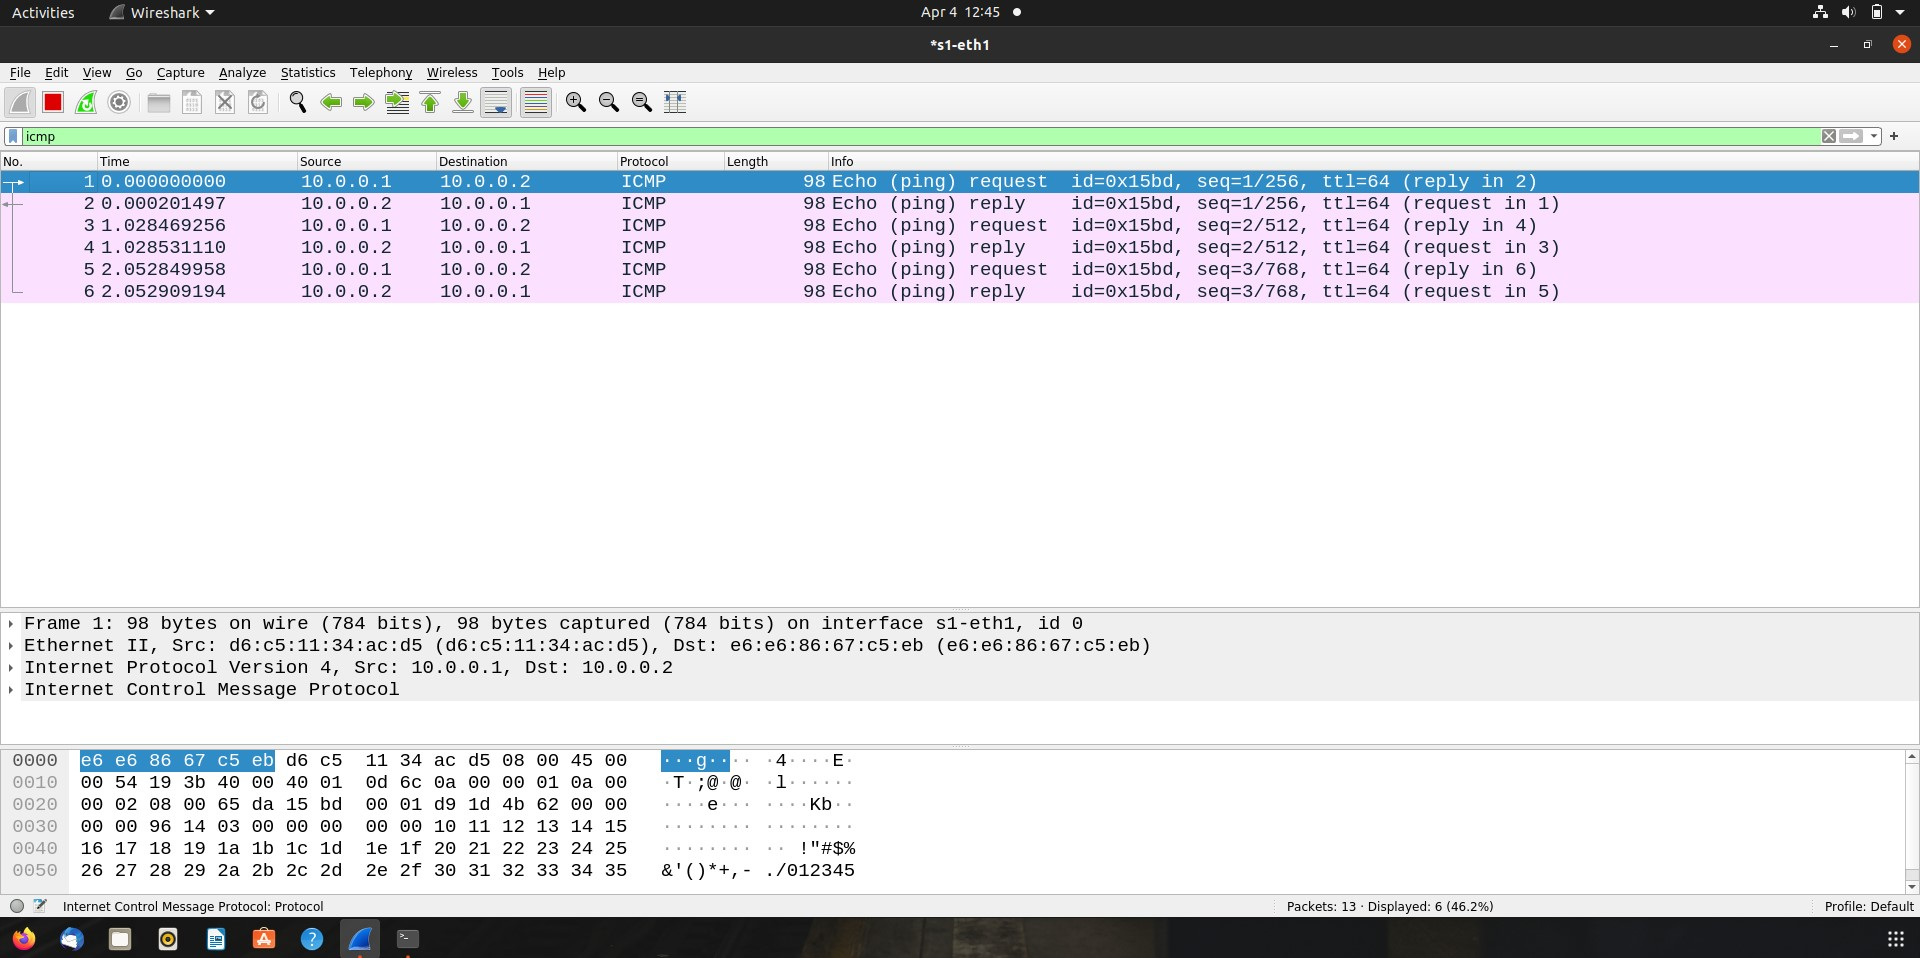
\includegraphics[width=1.0\textwidth]{figures/1g.jpg}
    \caption
	{
\lr{h1}، \lr{h2} را پینگ می‌کند.
	}
    \label{fig:fig1}
\end{figure}
برای بسته‌های کپچر شده در وایرشارک از پروتکل \lr{ICMP} استفاده شده است. از آنجایی که پینگ با 3 پکت انجام شده است (هاست \lr{h1} 3 پکت را برای \lr{h2} ارسال می‌کند)، وایرشارک 3 پکت برای \lr{request} و 3 پکت برای \lr{reply} را نمایش می‌دهد. در واقع به ازای هر پکتی \lr{request}ِ که \lr{h1} ارسال می‌کند، دریافت پیغام \lr{reply} آن به معنی برقرار بودن ارتباط بین دو هاست است.
\section{}
\begin{figure}[H]
    \centering
    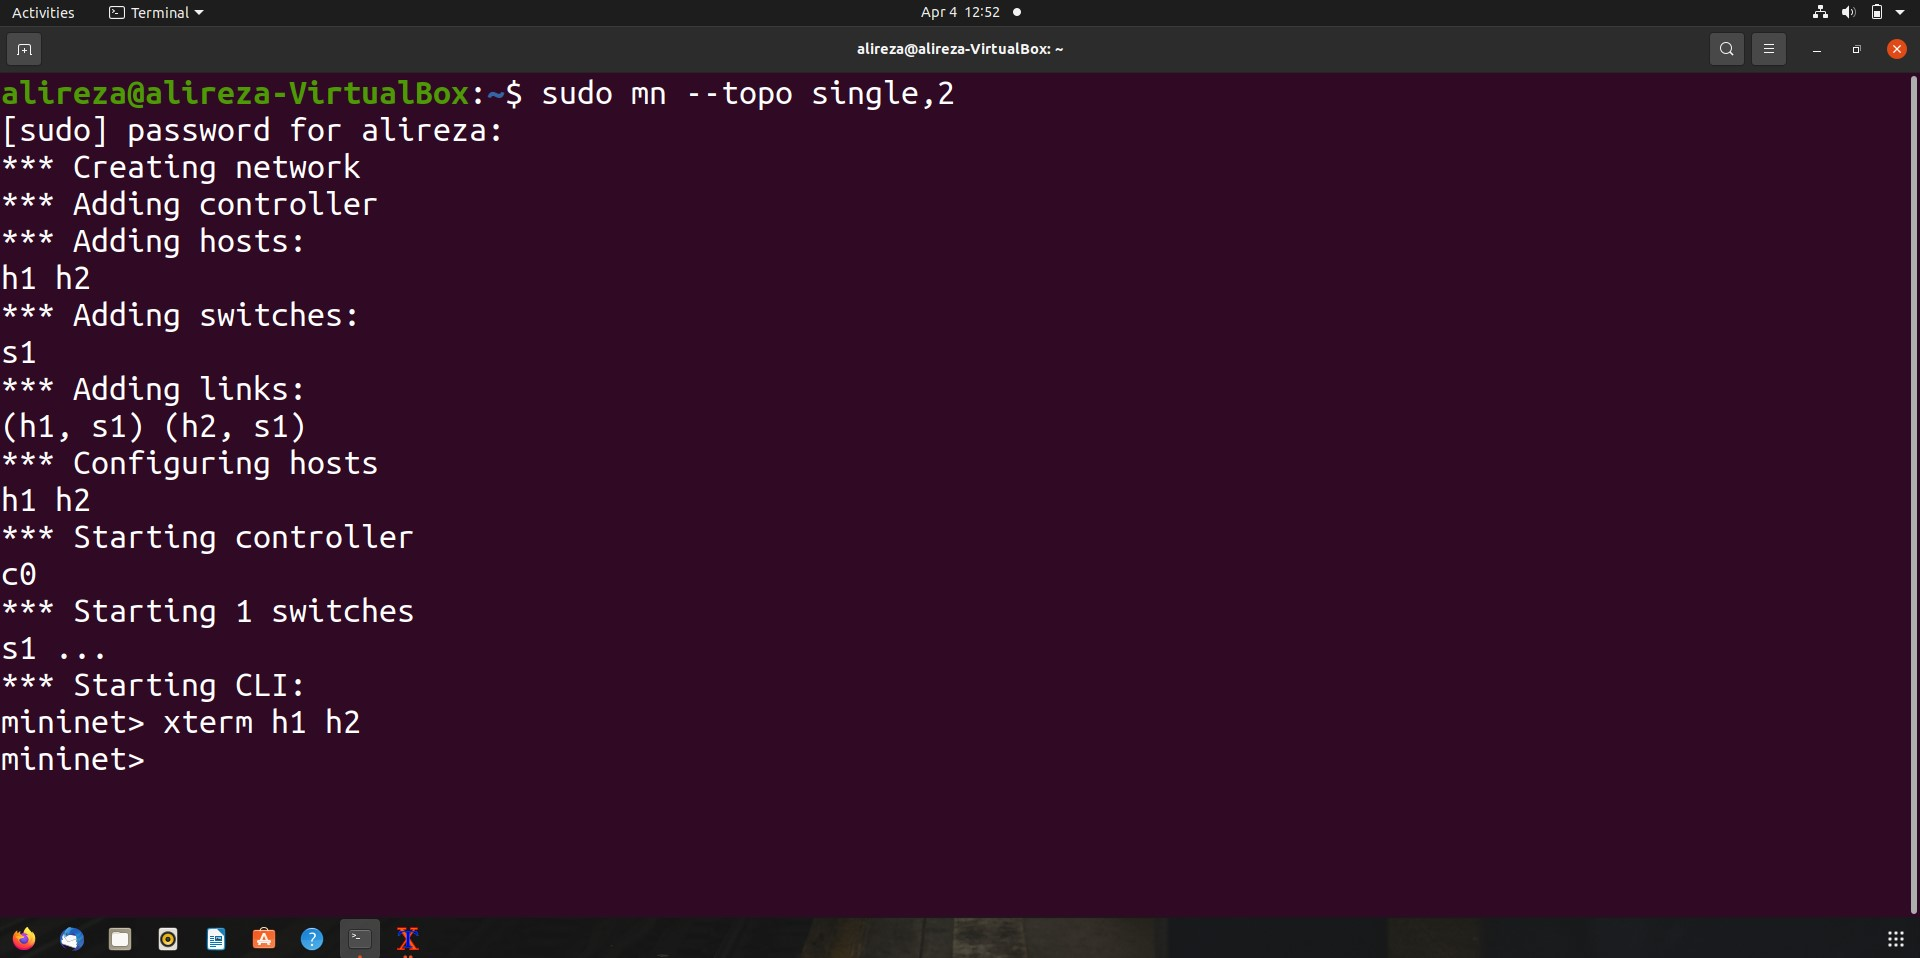
\includegraphics[width=1.0\textwidth]{figures/2a.jpg}
    \caption
	{
یک توپولوژی ساده با دو هاست را ایجاد می‌کنیم.
	}
    \label{fig:fig1}
\end{figure}
\begin{figure}[H]
    \centering
    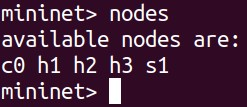
\includegraphics[width=1.0\textwidth]{figures/2b.jpg}
    \caption
	{
با دستور \lr{xterm} دو ترمینال جدا برای دو هاست \lr{h1} و \lr{h2} باز می‌کنیم.
	}
    \label{fig:fig1}
\end{figure}
\begin{figure}[H]
    \centering
    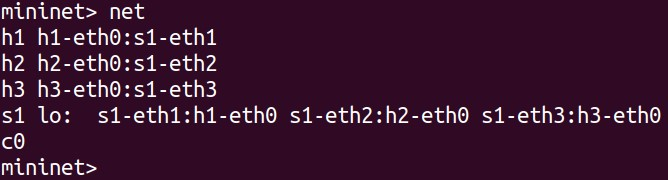
\includegraphics[width=1.0\textwidth]{figures/2c.jpg}
    \caption
	{
با دستور بالا یک سرور \lr{TCP} در \lr{h1} روی پورت 5000 به کار می‎‌اندازیم. همچنین در هر ثانیه نتایج مانیتور می‌شوند.
	}
    \label{fig:fig1}
\end{figure}
\begin{figure}[H]
    \centering
    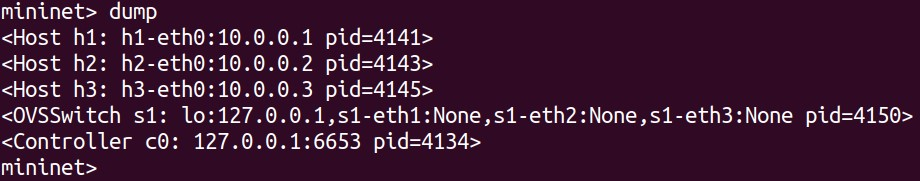
\includegraphics[width=1.0\textwidth]{figures/2d.jpg}
    \caption
	{
با دستور بالا یک کلاینت \lr{TCP} در \lr{h2} آغاز به کار می‌کند به سرور \lr{TCP} (که آدرس آن با دستور \lr{ifconfig} به دست می‌آید) متصل می‌شود. همچنین مدت زمان انتقال هم روی 20 ثانیه با آپشن \lr{-t} تنظیم شده است. همانطور که در تصویر می‌بینیم، از 0 تا 20 ثانیه، \lr{throughput} میانگین برابر \lr{17.0 Gbits/sec} است.
	}
    \label{fig:fig1}
\end{figure}

همچنین برای کشیدن نمودار می‌توانیم نتایج دستورات را درون فایل ذخیره کنیم و با استفاده از \lr{gnuplot} نمودار بکشیم. در نهایت برای تست شبکه روی حالت \lr{UDP}، از آپشن \lr{-u} استفاده می‌کنیم.


%%%%%%%%%%%%%%%%%%%%%%%%%%%%%%%%%%%
%%%%%%%%%%%%%%%%%%%%%%%%%%%%%%%%%%%
%%%%%%%%%%%%%%%%%%%%%%%%%%%%%%%%%%%

\section*{منابع}
\renewcommand{\section}[2]{}%
\begin{thebibliography}{99} % assumes less than 100 references
%چنانچه مرجع فارسی نیز داشته باشید باید دستور فوق را فعال کنید و مراجع فارسی خود را بعد از این دستور وارد کنید


\begin{LTRitems}

\resetlatinfont

\bibitem{b1} https://www.brianlinkletter.com/2015/09/how-to-map-openflow-switch-tcp-ports-in-mininet-sdn-simulations/
\bibitem{b1} https://neelshelar.com/openflow-protocol-importance-message-types/
\bibitem{b1} http://csie.nqu.edu.tw/smallko/sdn/iperf\_mininet.htm


\end{LTRitems}

\end{thebibliography}


\end{document}
